\subsection{Database Design}

Projektets database har gruppen valgt at hoste i lokal storage. Dette er valgt da der under semesterets forløbet opstod problemer med skolens licens af Microsoft produkter. For at undgå at komme ud for udfordringer med hosting senere i forløbet, blev der valgt at gå med den sikre løsning, at hoste databasen lokalt på enheden. Til dette benyttede gruppen et docker image, specifikt det samme image som blev benyttet i DAB undervisning, til vores SQL server.
%(https://docs.microsoft.com/en-us/sql/linux/quickstart-install-connect-docker?view=sql-server-ver15&preserve-view=true&pivots=cs1-powershell)
Hvis ikke der var problemer microsoft, havde gruppen i stedet valgt at lagre data på en cloud-based storage fremfor lokal storage.\\



For at kunne udarbejde et ER diagram til modellering af vores sql database skal vi start med at finde ud af hvilke krav vi har til og hvilke attributter vi ønsker at gemme i vores database.
Først og fremmest ønskede grupper at vi kunne gemme beskrivelserne af de forskellige rum, i spillets layout, for at formindske antallet af filer i klienten, og samtidigt gøre eventuelle senere tilføjelser nemmere.\\ 
Her benyttes rummets id som key, da vi ikke ønsker at man skal kunne oprette flere beskrivelser til samme rum.

\begin{figure}[H]
\centering
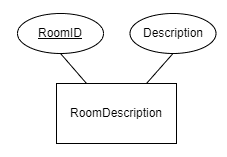
\includegraphics[width = 0.5\textwidth]{02-Body/Images/ER-RoomDescription.PNG}
\caption{ER diagram for Roomdescription. En beskrivelse består blot af en beskrivende string samt det tilhørende unikke rumid.}
\label{fig:ER-Roomdescription}
\end{figure}

Her efter kommer kravene til at kunne gemme et spil for en bruger. Her ønskede vi at man kunne stå et vilkårligt sted i spillet, med untagelse af en combat, og gemme spillet. Det skulle derefter være muligt for spilleren at loade spillet igen, hvorefter spillet er i samme stadie som man gemte det i.

\begin{figure}[H]
\centering
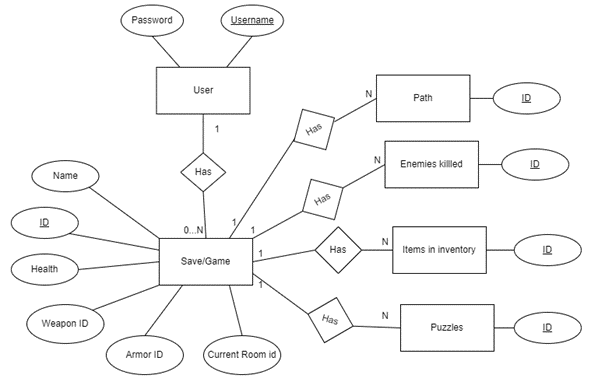
\includegraphics[width = \textwidth]{02-Body/Images/ER-GameSave.PNG}
\caption{ER Diagram til at gemme et spil til en specifik bruger}
\label{fig:ER-GameSave}
\end{figure}

Først og fremmest ønskede gruppen et bruger system, så eventuelle gemte spil kun tilhørte en bruger.
Der gemmes derfor en bruger entitet med et unikt brugernavn og et tilhørende password.
Sikkerhed på password og versalfølsomhed på brugernavnet håndteres af spillets backend.\\
En spiller skal derefter kunne gemme unikke 5 spil med forskellige oplysninger.
Restriktionen med max 5 forskellige spil pr. Bruger, håndteres ved at oprette 5 "tomme" gemte spil ved oprettelsen af en bruger.
Et af disse gemte spil overskriver derfor når vi gemmer. Der kan på denne måde ikke oprettes mere en 5 gemte spil pr. bruger.\\
I et gemt spil ønkede vi at gemme en række forskellige attributter for spilleren.
Første og fremmest får hver spil et unikt id som vi benytter til identifikation og at lave forhold mellem de forskellige tabeller.
Et gemt spil får et navn, valgt af brugeren, som gør det nemmere for brugeren at differentiere mellem de forskellige spil. \\ Dette navn skal være forskelligt fra de 4 andre gemte spil som tilhører samme bruger.\\
En spiller Health gemmes også, da man kan have taget skade efter en kamp.\\
Det gemmes også hvilket rum, spilleren står i når spillet gemmes, så vi loader korrekt tilbage. 
En spiller kan derudover også holde genstande, som armor og våben, i hånden eller i sit inventory. Dette gemmes også henholdsvist som en del af et spil og i en inventory liste tilhørende spillet. 

Tabellen med inventory har 2 atributter, et ID, som svarer til en bestemt genstand, og en reference til set SaveID. Denne parring er unik, da man ikke kan holde 2 af den samme genstand.\\
Tabellerne med Enemies og puzzles fungerer på samme måde. Her har hver enemy og puzzle i spillet et unikt id. Id’et gemmes i kombination med et saveId, som et unikt par, da man ikke kan vinde over samme enimy og løse samme puzzle flere gange.\\
Til slut ønskede vi at kunne vise spilleren de rum som allerede er blevet besøgt. Derfor gemmes der i path tabellen, for hvert spil, en unik kombination af saveID og besøgte rum id. Denne parring er unik da man blot behøver at besøge et rum en gang, før det er synligt på kortet. 

Der er i projektet oprettet klasser tilsvarende ER diagrammerne.
Forholdene mellem disse, samt keys, er opsat i DaG-db klassen og er skrevetved hjælp af fluentAPI. Dette kan ses i Implementationsafsnmittet.
